\chapter*{Die Autoren}
%%% Abkürzung in der Kopfzeile
%Kopfzeile linke Seite
	\lehead{Die Autoren} \cehead{}\rehead{}
%Kopfzeile rechte Seite
	\lohead{}\cohead{}\rohead{Die Autoren}

\parpic[l]{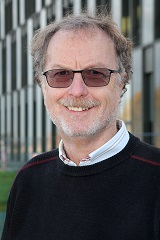
\includegraphics[angle=0,scale=0.6]{Bilder/Hermann.jpg}}
\noindent\textbf{Prof. Dr. rer. pol. Hermann-Josef Kruse}\\
Fachhochschule Bielefeld\\
Fachbereich Ingenieurwissenschaften und Mathematik\\
\href{mailto:hermann-josef.kruse@fh-bielefeld.de}{hermann-josef.kruse@fh-bielefeld.de}
\\ \\
\textbf{Fachgebiete:} Wirtschaftsmathematik, Operations Research
\\ \\
Seit 1995 als Professor für Wirtschaftsmathematik (insbesondere Operations Research) an der Fachhochschule Bielefeld tätig und lehrt dort im Bachelor-Studiengang \textit{Angewandte Mathematik} und im Master-Studiengang \textit{Optimierung \& Simulation} des Fachbereichs \textit{Ingenieurwissenschaften \& Mathematik}. Gründungsmitglied des Forschungsschwerpunktes \textit{Angewandte Mathematische Modellierung \& Optimierung} (FSP AMMO) der FH Bielefeld. F\&E-Projekte im Bereich der Optimierung und Simulation diskreter Systeme zur Entscheidungsunterstützung bei betrieblichen Problemstellungen.
\\ \\
N.N.



